\documentclass[a4paper,14pt]{article} % тип документа
%\documentclass[14pt]{extreport}
\usepackage{extsizes} % Возможность сделать 14-й шрифт


\usepackage{geometry} % Простой способ задавать поля
\geometry{top=25mm}
\geometry{bottom=35mm}
\geometry{left=20mm}
\geometry{right=20mm}

\setcounter{section}{0}

%%%Библиотеки
%\usepackage[warn]{mathtext}
%\usepackage[T2A]{fontenc} % кодировка
\usepackage[utf8]{inputenc} % кодировка исходного текста
\usepackage[english,russian]{babel} % локализация и переносы
\usepackage{caption}
\usepackage{listings}
\usepackage{amsmath,amsfonts,amssymb,amsthm,mathtools}
\usepackage{wasysym}
\usepackage{graphicx}%Вставка картинок правильная
\usepackage{float}%"Плавающие" картинки
\usepackage{wrapfig}%Обтекание фигур (таблиц, картинок и прочего)
\usepackage{fancyhdr} %загрузим пакет
\usepackage{lscape}
\usepackage{xcolor}
\usepackage{dsfont}
%\usepackage{indentfirst}
\usepackage[normalem]{ulem}
\usepackage{hyperref}




%%% DRAGON STUFF
\usepackage{scalerel}
\usepackage{mathtools}

\DeclareMathOperator*{\myint}{\ThisStyle{\rotatebox{25}{$\SavedStyle\!\int\!\!\!$}}}

\DeclareMathOperator*{\myoint}{\ThisStyle{\rotatebox{25}{$\SavedStyle\!\oint\!\!\!$}}}

\usepackage{scalerel}
\usepackage{graphicx}
%%% END 

%%%Конец библиотек

%%%Настройка ссылок
\hypersetup
{
colorlinks=true,
linkcolor=blue,
filecolor=magenta,
urlcolor=blue
}
%%%Конец настройки ссылок


%%%Настройка колонтитулы
	\pagestyle{fancy}
	\fancyhead{}
	\fancyhead[L]{Домашнее задание}
	\fancyhead[R]{Крейнин Матвей, группа Б05-005}
	\fancyfoot{}
    \fancyfoot[C]{\thepage}
    \fancyfoot[R]{ТРЯП}
%%%конец настройки колонтитулы



\begin{document}
%%%%Начало документа%%%%

\section{Задание 3}
\subsection{Задача 1}
    Рассмотрим пример автоматов с картинок.
   
    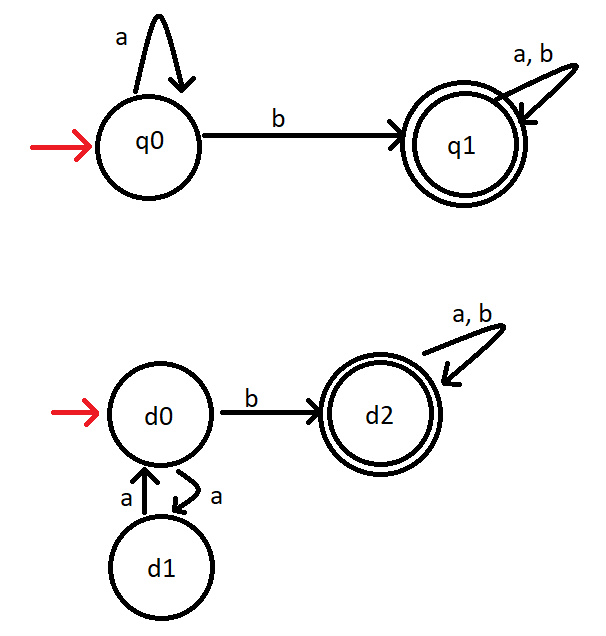
\includegraphics[scale = 0.7]{01.png}
   
    По предложенному способу построения автомата, получаем автомат:

    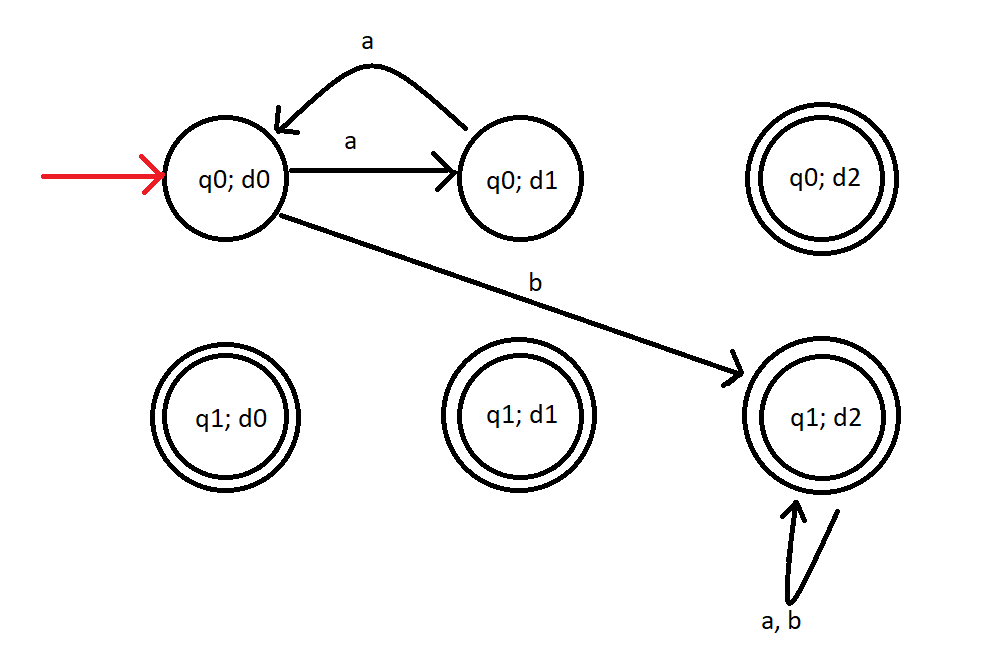
\includegraphics[scale = 0.7]{02.png}

    Можно заметить, что слово ab не будет принято этим автоматом, т.к. сначала он перейдет в состояние ($q_0$, $d_1$), из которого нет перехода по b.
    Следовательно слово ab не будет принято, хотя оно распознается первым автоматом, как валидное.
    
    Поэтому ответ: Нет, неверно. 

\subsection{Задача 2}
\textbf{a)} Докажем это утверждение по индукции, 

База для |$\omega$| = 0. Автомат должен распознавать слово, поэтому у него должно быть хотя бы одно принимающее состояние. 
        
|$\omega$| = 1. Автомат для этого случая строится тривиально. Рассмотрим суффикс a. По букве a он переходит в принимающее состояния, по букве b остается в начальном. Из принимающего по букве a остается в принимающем, по букве b возвращается в начальное.
База доказана.

Тогда для |$\omega$| $=$ n. По предположению нам нужно n состояний автомат. У нас появилась еще одна буква, по которой должен вести в новое состояние, иначе если оно ведет уже которое было, то можно будет привести контрпример с длиной суффикса меньше, чем |$\omega$|.

\underline{Доказано.}
\vspace{5mm}

\textbf{б)} Построим такой автомат $\mathcal{A}$. 
$Q = \{ q_0, q_1, ..., q_n \}$  $F = q_n$, $q_0$ - начальное состояние.
А алфавит выберем $\Sigma = \{0, 1\}$ между ним и алфавитом $\Sigma = \{a, b \}$ можно построить биекцию.
Суффикс выглядит так: $m_{[0]}m_{[1]}...m_{[n-1]}$
Функция перехода будет устроена так: $\delta(q_0, \overline{m_{[0]}}) = q_0$

$\delta(q_i, m_{[i]}) = q_{i + 1}$

$\delta(q_i, \overline{m_{[i]}}) = q_{k}$

Определим, что такое $q_k$. Пусть мы считали r букв, тогда мы этот массив из r букв сравниваем с суффиксом m, ища максимальное вхождение этого в массив в начало нашего суффикса.
Сравнивая наши буквы массива и суффикса следующим образом: последнюю букву массива с первой буквы суффикса, предпоследнюю букву со второй буквой суффикса.
Получаем, что k это позиция, до которой есть вхождение в суффикс k.

Теперь докажем, что автомат принимет слова с суффиксом $m$, а других не принимает.

Пусть автомат находится находится в $q_i$, то принимаю букву $m_{[i+1]}$ он переходит в состояние $q_{i+1}$, это следует из определения функции $\delta$.
Таким образом, принимая последовательно буквы $m_{[i+1]}, ..., m_{[n]}$, автомат перейдет в принимающее состояние.
Если в состоянии $q_i$ приходит $\overline{m_{[i+1]}}$ или в принимающем состоянии приходит еще одна буква, то автомат ищет максимальное наложение слова на суффикс.
Тогда автомат переходит в новое состояние $q_{l+1}$ и продолжает поиск считывание букв. Если подано слово без суффикса m, то автомат не дойдет до принимающешго состояния $q_n$, следует из определения функции перехода.

\underline{Доказано.}

\subsection{Задача 3.}
Можем представить это язык в виде: $(a|b)^{n-i}$ a $(a|b)^{i-1}$.
Можем представить это слово, как суффикс, у которого есть a на n-i+1 позиции. Тогда получаем, что у нас $2^{i-1}$ различных состояний после а и $2^{n-i}$ различных состояний до а.
Получаем количество различных суффиксов, которые мы можем сотавить будет равно $2^{n-i} \cdot 1 \cdot 2^{i-1}$ = $2^{n-1}$. По доказанной задаче 2 на каждый суффикс приходится n + 1 состояние.
И тогда получаем $2^{n- 1} \cdot (n+1)$. 

$2^n \leq  2^{n-1} \cdot (n+1)$, а это верно для всех 1 $\leq n$, а это верно из условия задачи. 

\underline{Доказано.}


\end{document}